This section will describe the hardware component of the project and explain 
the rationale for some important design decisions including component selection,
schematic design, and component placement on the PCB. It will also detail any 
variations from what was planned in the project proposal and why these changes
were made.

\subsection{Component Selecton}

We considered a number of requirements in choosing a microcontroller for our
project. We identified several microcontroller features that were needed to
support our project requirements and did not consider any microcontrollers
without these features. These features are:
\begin{itemize}
    \item Bluetooth Low Energy support
    \item At least one I2C master mode interface for sensors
    \item An SPI or SD/MMC interface to connect and SD card
\end{itemize}

While we could have selected from a much wider variety of microcontrollers if we
had considered using a separate Bluetooth LE controller chip, we chose to limit
our selection to parts that featured an integrated Bluetooth LE radio. This is
to reduce part count (and therefore size, cost and design complexity) and to
provide better power consumption.

Table \ref{tab:mcu-comp-general} shows a brief summary of the microcontroller
options that we considered, all of which meet the minimum criteria outlined
above. The costs listed in the table are the price in Canadian dollars in single
quantities in the friendliest device package available and cut tape or tray
packaging from digikey.ca. These prices are often volatile and are therefore
listed here only for relative comparison.

All of the parts listed are based on ARM cortex processors. Nordic
Semiconductor's nRF5340 and the Silicon Labs EFR32BG22C224 use a Cortex-M33
while all of the other microcontrollers listed use a Cortex-M4. We estimated that
any of these microcontrollers would have sufficient processor performance for
our application. Similarly, all of the listed options have ample flash storage
and SRAM.

Not all of the listed microcontrollers come in packages that are easy to solder
by hand. The relatively small QFN packages of the nRF52832 and EFR32BG22C224 can
be soldered with relative ease using a hot air reflow station or an iron and be
inspected easily with a microscope. Unfortunately the other options are much
more difficult, the Apollo3 Blue's BGA package and the WLP package of the
MAX32668 each have a large array of solder balls. These packages can be soldered
with hot air reflow, but we did not have the equipment to inspect them. The
nRF52840 and nRF5340 are a middle ground, their aQFN packages have many fewer
balls, but they still do have two rows of connections. This means that while we
are able to solder the packages with hot air reflow they would difficult to
inspect. Another option that was considered to sidestep the issue of soldering 
difficulty entirely was the use of modules that integrate the microcontroller and
a pcb antenna on a small pcb. The nRF52840 and nRF52830 can be found in these 
modules and the Apollo3 Blue is available in a similar module from SparkFun 
branded as SparkFun Artemis.

The availability was also a limiting factor in our decision. Most of our listed
microcontrollers were readily available from a variety of online component
vendors. The exception was the Apollo3 Blue, which was not readily available
outside of SparkFun's Artemis module, and the MAX32668 which is a newly
available part and could only be ordered as a sample from Maxim's
website.

\begin{table*}[htb]
\centering
\begin{tabular}{>{\centering\arraybackslash}m{2.2cm}|
                >{\centering\arraybackslash}m{2.5cm}|
                >{\centering\arraybackslash}m{2.0cm}|
                >{\centering\arraybackslash}m{1.5cm}|
                >{\centering\arraybackslash}m{1.2cm}|
                >{\centering\arraybackslash}m{1.8cm}|
                >{\centering\arraybackslash}m{1.2cm}}
\toprule
Part Number & Manufacturer & CPU & Program Memory & SRAM & Friendliest Package & Cost \\
\midrule
nRF52840 & Nordic Semiconductor & ARM Cortex-M4 at 64 MHz & 1 MiB & 256 KiB  & aQFN73 & \$9.34 \\
nRF52832 & Nordic Semiconductor & ARM Cortex-M4 at 64 MHz & 512 KiB & 64 KiB  & QFN48 & \$8.19 \\
nRF5340 & Nordic Semiconductor & Dual ARM Cortex-M33 at 96/64 MHz & 1 MiB & 512 KiB & aQFN94 & \$13.85 \\
Apollo3 Blue & Ambiq & ARM Cortex-M4 at 48 MHz & 1 MiB & 384 KiB & BGA81 & N/A \\
MAX32668 & Maxim Integrated & ARM Cortex-M4 at 96 MHz & 1 MiB & 560 KiB & WLP109 & N/A \\
EFR32BG22 C224 & Silicon Labs & ARM Cortex-M33 at 76.8 MHz & 512 KiB & 32 KiB & QFN40 & \$5.26 \\
\bottomrule
\end{tabular}
\caption{Comparison of Microcontrollers With Bluetooth Low Energy Radios}
\label{tab:mcu-comp-general}
\end{table*}

Table \ref{tab:mcu-comp-comm} compares the communications interfaces available
on the microcontrollers we considered. All of the micrcrocontrollers feature at
least Bluetooth Low Energy 5.0, at least two I2C interfaces and at least two SPI
interfaces. In addition to these interfaces the MAX32668 has an SD/MMC interface
controller which supports the SD3.0 specification. This interface would allow
significantly faster SD card access speeds than we can accomplish using an SPI
interface.

The nRF52840 and MAX32688 both feature USB interfaces. We decided to have a USB
CDC-ACM interface for debugging and as a wired alternative to the
Bluetooth interface for data transfer. While we could have implemented a USB
interface with any of the microcontrollers listed by using a separate USB to
UART chip, using one of the microcontrollers with a built-in USB interface 
gives us greater integration saving us cost, board space, complexity and
power usage.

\begin{table*}[htb]
\centering
\begin{tabular}{>{\centering\arraybackslash}m{3.0cm}|
                >{\centering\arraybackslash}m{1.8cm}|
                >{\centering\arraybackslash}m{1.8cm}|
                >{\centering\arraybackslash}m{1.8cm}|
                >{\centering\arraybackslash}m{1.5cm}|
                >{\centering\arraybackslash}m{3.0cm}}
\toprule
Part Number & I2C Master Interfaces & SPI Master Interfaces & SD/MMC Interface & BLE Version & USB \\
\midrule
nRF52840 & 2 & 4 & None & 5.2  & 2.0 Full Speed \\
nRF52832 & 2 & 3 & None & 5.2  & None \\
nRF5340 & 4 & 5 & None & 5.1 & None \\
Apollo3 Blue & 6 & 6 & None & 5.0 & None \\
MAX32668 & 3 & 3 & SD3.0 & 5.0 & 2.0 High Speed \\
EFR32BG22C224 & 2 & 2 & None & 5.2 & None \\
\bottomrule
\end{tabular}
\caption{Comparison of Microcontroller Communications Hardware}
\label{tab:mcu-comp-comm}
\end{table*}

While our project did not necessarily require hardware accelerated cryptography,
we thought it should be included to accomodate any future software layers that 
build on top of our platform. Since the device collects information about the 
user it is likely that cryptography would be heavily used by security features,
and software implementations of the cryptographic alrogithms may not be adequate.  
Table \ref{tab:mcu-comp-crypto} shows the cryptography features of the 
microcontrollers that we considered. All of the microcontrollers have suitable 
hardware accelerated cryptography features with the exception of the nRF52832 
which lacks any modular arithmetic acceleration for public key cryptography and 
the Apollo3 Blue which has no hardware cryptography accelerator.

\begin{table*}[htb]
\centering
\begin{tabular}{>{\centering\arraybackslash}m{2.5cm}|
                >{\centering\arraybackslash}m{2.0cm}|
                >{\centering\arraybackslash}m{2.0cm}|
                >{\centering\arraybackslash}m{2.5cm}|
                >{\centering\arraybackslash}m{2.5cm}|
                >{\centering\arraybackslash}m{1.5cm}}
\toprule
Part Number & Hashes & Public Key Algorithms & Symmetric Key Algorithms & AES Modes & True Random Number Generator \\
\midrule
nRF52840 & SHA-1, SHA-2 up to 256 bits, HMAC & RSA up to 2048 bit key, ECC & AES128, ChaCha20, Poly1305 & ECB, CBC, CMAC/CBC-MAC, CTR, CCM/CCM* & Yes \\
nRF52832 & None & None & AES128 & ECB, CCM & No \\
nRF5340 & SHA-1, SHA-1 up to 256 bits, HMAC & RSA up to 3072 bit key, ECC & AES128, AES256 & ECB, CBC, CMAC/CBC-MAC, CTR, CCM/CCM*, GCM & Yes \\
Apollo3 Blue & None & None & None & None & No \\
MAX32668 & SHA-2 up to 512 bits & RSA up to 4096 bit key, ECC & AES128, AES192, AES256, DES, 3DES & ECB, CBC, CFB, OFB, CTR & Yes \\
EFR32BG22 C224 & SHA-1, SHA-2 up to 256 bits & ECC & AES128, AES192, AES256 & ECB, CTR, CBC, CFB, GCM, CBC-MAC, GMAC, CCM & Yes \\
\bottomrule
\end{tabular}
\caption{Comparison of Microcontroller Cryptography Hardware}
\label{tab:mcu-comp-crypto}
\end{table*}

Because of its availability, relatively easy to work with package, suitable
serial interface, integrated USB support and hardware cryptography acceleration
we chose to use the nRF52840 microcontroller. The Apollo3 Blue had tempting low 
power features, but questionable availability and a complete lack of hardware 
accelerated cryptography. The MAX32668 would also have been a very strong 
option, but it is not yet widely available. The EFR32BG33C224's lack of an 
integrated USB interface and comparatively little documentation caused us to
choose the nRF52840 over it.

More specifically, it was decided to use a module (BMD-340) containing the
nRF52840 instead of the bare chip itself. This decision was made because 
the module is much more available for purchase, it has a built in Bluetooth 
antenna which has already been certified by several different parties, it is 
easier to solder, and it includes several supporting components for the 
microcontroller such as oscillators and capacitors. The module is more 
expensive and larger than the microcontroller by itself, however when taking 
into consideration the size and cost of the additional components it contains, 
it likely as good or better than using individual components.

The selection of sensors that made it into the final design are an inertial 
measurement unit (IMU), a heart rate sensor, an air quality sensor, a UV light 
sensor, an infrared temperature sensor and an ambient temperature sensor. This 
suite of sensors was selected in order to capture as much information as 
possible without increasing the cost of the device too much. The component 
choice for each of these sensors was mostly driven by cost, availability, and 
ease of soldering. Taking these factors into consideration narrowed down the 
options very quickly. The infrared temperature sensor and ambient temperature 
sensor are both integrated into the same component. The ambient temperature 
sensor will indicate the temperature of the user’s environment while the 
infrared temperature sensor measures the user’s body temperature. The air 
quality sensor and UV light sensor will provide additional information about 
the user’s environment. The IMU will provide information about the user’s 
movements, and the heart rate sensor will measure the user’s heart rate. A 
listing of the exact components used for each of these sensors is provided 
below.

\begin{itemize}
   \item ICM-20948: Inertial Measurement Unit (IMU)
   \item MAX86150EFF+T: Heart rate sensor
   \item ZTP-148SR: Infrared and ambient temperature sensor
   \item BME680: Air quality sensor
   \item SI1133-AA00-GM: UV light sensor
\end{itemize}

\subsection{Schematic}

The schematic is split into three major sections. These are the power supply, 
processor, and sensors. The power supply is responsible for managing the 
devices internal lithium-ion polymer (LiPo) battery and powering all other 
parts of the circuit. When the device has its USB-C port connected to a 
suitable host, the power supply will shift the electrical load from the 
internal battery to the USB power source and begin charging the internal 
battery. When USB power is lost charging stops and the electrical load is 
shifted back to the internal battery. Transitions between the two power 
sources are seamless and will not interrupt operation of the rest of the 
device. Upon request by the processor, the power supply can also perform fast 
charging of the battery. The processor is responsible for communicating with 
all onboard sensors and the internal SD card through several I2C and SPI 
busses. Communication with the outside world is also handled by the processor 
through the USB-C port or wirelessly over Bluetooth. The collection of onboard 
sensors is responsible for gathering information about the user and their 
environment to be used by the processor.

The implementation of the power supply was mostly guided by the requirements of 
the rest of the system and cost. The majority of the components in the design 
require 1.8V to operate with the exceptions being the RGB status LED and the SD 
card requiring 3.3V. The status LED does not have a specific voltage 
requirement, but 1.8V was not sufficient to overcome the forward voltage of the 
diodes so 3.3V was used instead with appropriate series current limiting 
resistors. The choice of a LiPo battery meant that the power supply input 
voltage could be anywhere from 3.7V to 2.8V depending on state of charge, and 
when connected to USB power the input would be 5V. There were several ideas on 
how to build a power supply that would meet all the requirements, but the final 
decision is pictured in Figure \ref{fig:BlockDiagram_PowerSupply} as a block 
diagram.

\begin{figure}[!htb]
\centering
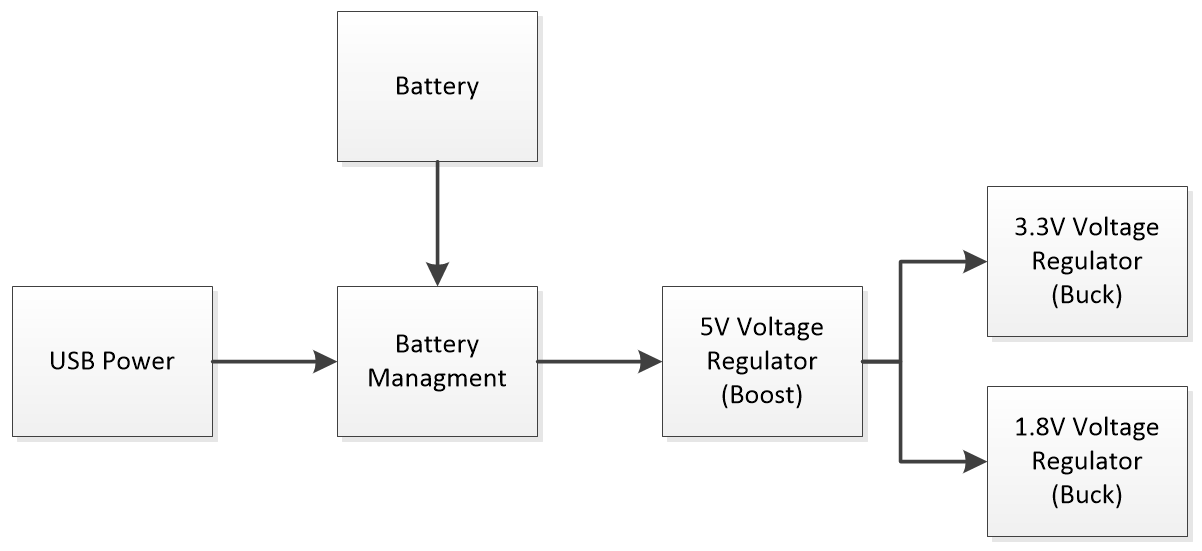
\includegraphics[width=\textwidth]{images/BlockDiagram_PowerSupply.png}
\caption{Block diagram of power supply.}
\label{fig:BlockDiagram_PowerSupply}
\end{figure}

The battery and USB power input are both connected directly to a dedicated 
battery management IC. This IC handles battery charging, battery protection, 
and automatic switchover from one power source to the other. It does not 
however provide any means of regulation. Regulation is handled by three 
separate voltage regulators, the first of which boosts the input up to 5V. The 
last two regulators step the output of the 5V regulator down to 3.3V and 1.8V. 
The intermediate 5V is not strictly necessary as 5V is not used anywhere in the 
design, but without it the 3.3V regulator would need to be a more expensive 
buck-boost type since the input voltage could be above or below its output. 
Additionally, the 5V regulator has an enable input that is used in conjunction 
with some soft power on/off circuitry to completely isolate the load from the 
power source and reduce standby power consumption to nearly zero. Another option 
that was considered was using the voltage regulator built into the chosen 
processor to generate the 1.8V from 3.3V. It was ultimately decided not to go 
this route due to concerns over robustness and maximum current limitations. With 
the current design, both the 3.3V and 1.8V regulators can operate independent of 
each other, have short circuit protection with automatic recovery, have over 
temperature protection, can deliver much more current than needed, and should 
operate with over 90\% efficiency according to the device datasheets. The result 
is a very robust, safe, and cheap solution that integrates well with the rest of 
the design.

One interesting design feature related to the power supply is the way in which 
the device is powered on and off. The most obvious approach was to use a simple 
on/off switch that connects or disconnects power from the load, but some flaws 
were identified with this idea. Suddenly removing power from the microcontroller 
during writes to the SD card or communication over USB or Bluetooth may cause 
data corruption. Also, if the battery is allowed to die completely with the 
switch left on the device may “flicker” on and off similar to an LED flashlight 
with a dead battery. The next obvious approach was to leave power permanently 
connected to the microcontroller and use a momentary push button to toggle 
between a very low power state and normal operation. This solution solves the 
data corruption problem but does not eliminate the possibility of power 
“flicker” with a dead battery, and also suffers from unnecessarily high standby 
power consumption since the device does not actually turn off. Elements of both 
approaches were used to come up with a design that solves all of these problems. 
When the device is off, the power source and load are completely isolated by 
disabling the 5V regulator shown in Figure \ref{fig:BlockDiagram_PowerSupply}. 
A momentary power button enables this regulator when pressed, turning on the 
device. As soon as the microcontroller starts up it uses one of its GPIO pins to 
latch the power supply on before the user releases the momentary button. The 
momentary button and GPIO pin are the inputs to a logical OR gate that controls 
the enable pin of the voltage regulator. This means that the device will stay 
powered up for as long as the microcontroller desires regardless of what the 
user does with the power button. A separate signal from the momentary button is 
routed to an input pin of the microcontroller so that it can determine when the 
user is pressing the button. If the user holds the button for an extended period 
of time the microcontroller will go through a shutdown routine ended by turning 
off the GPIO pin that latched the power supply on. As soon as the user releases 
the power button all power will be lost and the device is off. A simplified 
schematic view of this arrangement can be seen in 
Figure \ref{fig:BlockDiagram_OnOff} below.

\begin{figure}[!htb]
\centering
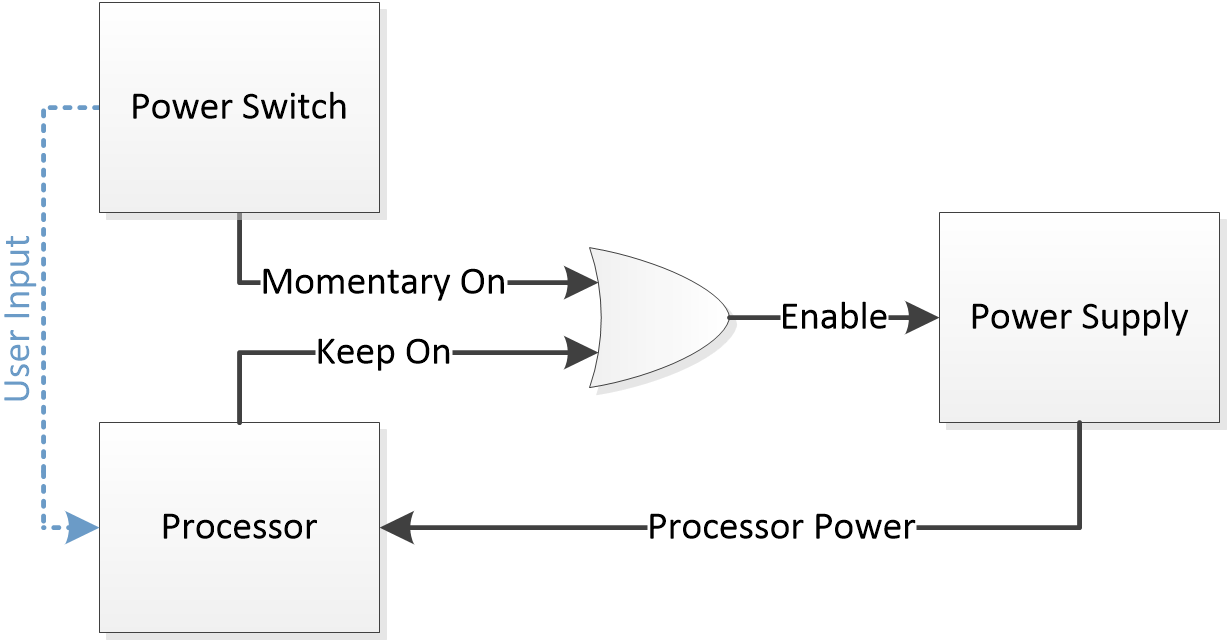
\includegraphics[width=\textwidth]{images/BlockDiagram_OnOff.png}
\caption{Simplified power on/off circuit.}
\label{fig:BlockDiagram_OnOff}
\end{figure}

The fact that the microcontroller can wait as long as it wants before turning 
itself off means that it can finish any pending IO without interruption and 
avoid data corruption. The “flicker” problem is also solved because the device 
can not turn on without the user pressing the button first. The isolation 
between power source and load when powered off means that standby power 
consumption should be extremely low. This implementation is slightly more 
complex and costly than the others because it uses some additional hardware 
components and relies on both hardware and software to work together, but it 
was decided that the benefits greatly outweigh the costs.

The implementation of the processor section of the schematic followed what was 
outlined in the proposal very closely. As described in 
the proposal, the design includes support for an SD card, USB communication, 
and Bluetooth communication to get data in and out of the device. All 
communication internal to the device between the microcontroller and other 
components is achieved with a combination of analog signals, GPIO pins, 
interrupt signals, I2C, and SPI. Figure \ref{fig:BlockDiagram_Processor} below 
is a block diagram showing how everything connects together.

\begin{figure}[!htb]
\centering
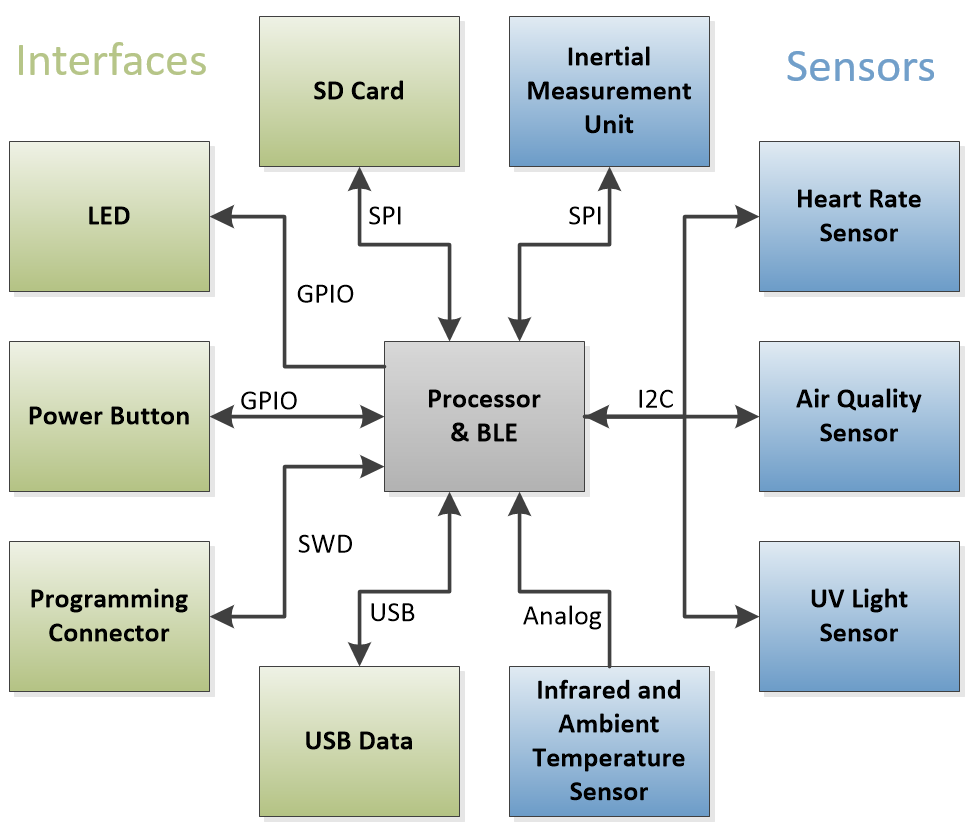
\includegraphics[width=\textwidth]{images/BlockDiagram_Processor.png}
\caption{Block diagram of processor and connected components.}
\label{fig:BlockDiagram_Processor}
\end{figure}

\subsection{PCB Layout}

The PCB design process completed with a 4-layer board measuring 35mm x 57mm as 
a result. All resistors and capacitors in the design use 0603 (Inch) size 
components because they are the smallest components available that we are
confident in being able to solder by hand. Figure \ref{fig:Board_TopBottom_Annotated}
shows an image of the circuit board as well as the locations of important 
components.

\begin{figure}[!htb]
\centering
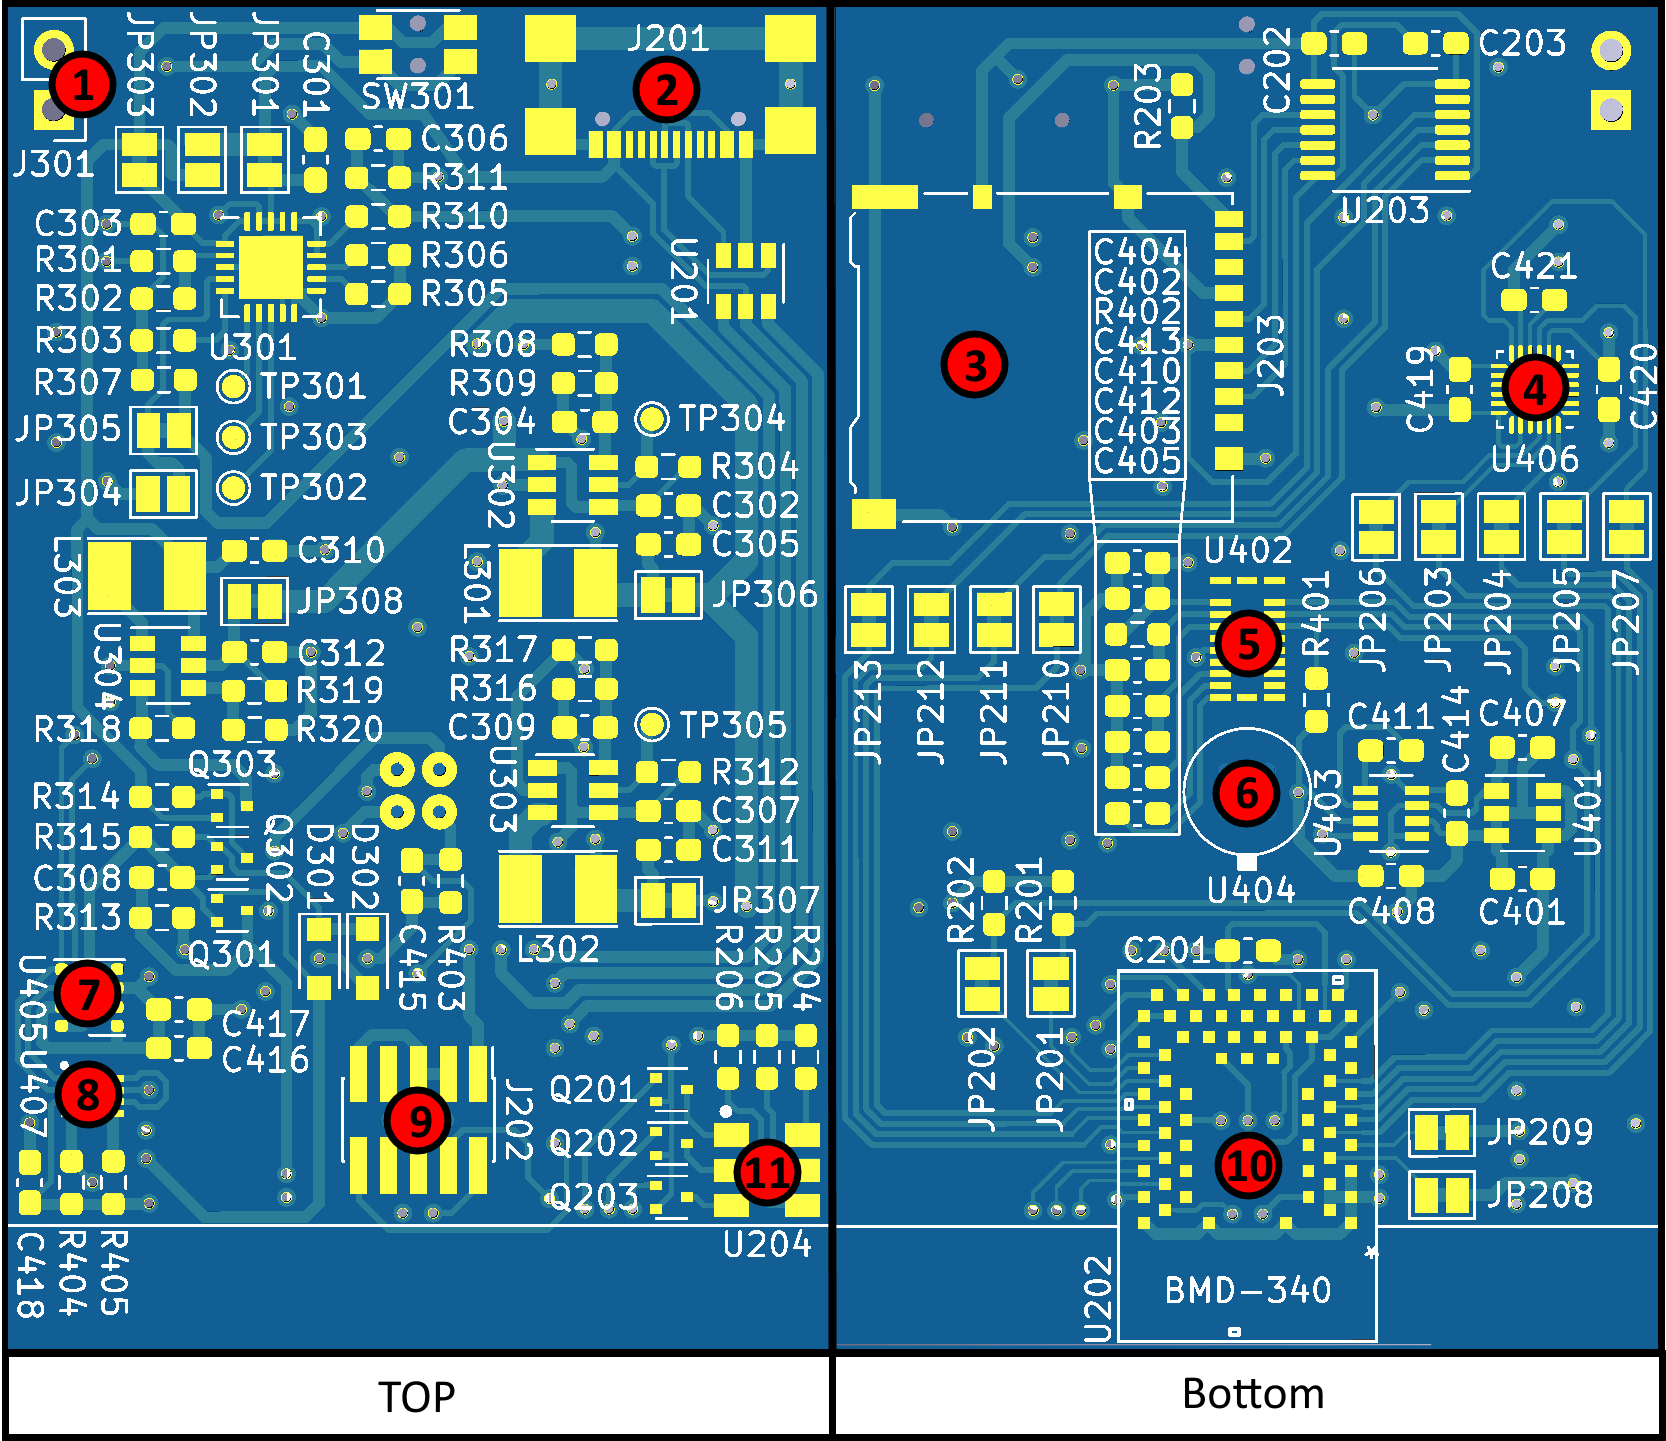
\includegraphics[width=\textwidth]{images/Board_TopBottom_Annotated.png}
\caption{CAD drawing of the completed PCB design.}
\label{fig:Board_TopBottom_Annotated}
\end{figure}

The following is a list of components indicated in Figure \ref{fig:Board_TopBottom_Annotated}: 
\begin{enumerate}
   \item LiPo battery connection
   \item USB-C port
   \item SD card slot 
   \item Inertial Measurement Unit (IMU)
   \item Heart rate sensor
   \item Infrared and ambient temperature sensor
   \item Air quality sensor
   \item UV light sensor
   \item SWD programming/debugging connector
   \item Processor module
   \item Status LED
\end{enumerate}

Placement of the components on the board was an important consideration. Many 
of them require proper positioning to work correctly. The USB port and SD card 
slot were placed near the edge of the board for easy access outside the 
enclosure. The heart rate sensor and infrared temperature sensor had to be 
placed on the bottom of the board so they could take measurements from the 
user’s arm. The LiPo battery will be placed on top of the board once it is 
assembled into the enclosure so that it does not block the heart rate sensor 
and temperature sensor. The status LED had to be on the top of the board so it 
could be seen by the user, but also had to be in a corner so it would not be 
covered by the battery. The air quality sensor needs access to air from outside 
the enclosure so it was placed near the edge of the board where some vents in 
the enclosure could be made. The UV light sensor had to placed on top of the 
board and also in a corner so it could receive light from outside the enclosure 
and not be blocked by the battery. The programming/debugging connector could 
have gone anywhere on the board, but the top was preferable so it could 
be accessed after the board was placed in the enclosure. The processor
module needed to have an entire edge of the board to itself, since 
recommendations from the manufacturer stated that the area around the Bluetooth 
antenna should be completely free of any metal in the PCB or elsewhere. These 
recommendations were followed closely to ensure that the Bluetooth 
communication works well in the final product. The final sensor to be placed 
was the IMU as it did not have any specific placement requirements.
